\chapter{مشخصات یک پایان نامه و گزارش علمی}
\section{مقدمه}
در این فصل، عملکرد مدل \lr{ProActionCLIP} در زمینه‌ی یادگیری پیوسته‌ی تشخیص حرکت انسان مورد ارزیابی قرار می‌گیرد. هدف از این ارزیابی، بررسی میزان صحت مدل در یادگیری وظایف جدید، ارزیابی میزان فراموشی دانش پیشین و تحلیل بهره‌وری محاسباتی آن از نظر مصرف سخت‌افزار و تعداد پارامترهای قابل‌آموزش است. به منظور ارزیابی جامع، مدل پیشنهادی با روش‌های مطرح در این حوزه مانند \lr{PIVOT} \cite{pivot}و سایر رویکردهای مرجع مقایسه می‌شود. برای این منظور، از مجموعه‌داده‌های نظیر \lr{UCF101} \cite{ucf101} و \lr{HMDB51} \cite{hmdb51} استفاده شده است.

در ادامه‌ی‌ این فصل، ابتدا معیارهای ارزیابی شامل صحت، میزان فراموشی معرفی می‌شوند. سپس، جزئیات مربوط به مجموعه‌های داده، تنظیمات آزمایشی، روش‌های مقایسه‌ای و تحلیل نتایج ارائه خواهد شد تا ارزیابی مدل پیشنهادی به‌طور کامل و شفاف صورت گیرد. در اخر نیز پیچیدگی محاسباتی بررسی خواهد شد. 
% سخت افزار رو تو همون پیچیدگی محاسباتی بگم. پارامتر. شامل حافظه . بگم رو جی پی یو فلان اموزش دادم. 

\section{معیار‌های ارزیابی}
در یادگیری پیوسته، دو معیار ارزیابی اهمیت دارند. یکی از آن‌ها میانگین صحت وظایف با وجود یادگیری سایر وظایف بوده و دیگری میزان فراموشی مدل پس از یادگیری هر وظیفه است که در ادامه هر یک شرح داده خواهد شد. 
 

\subsection{میانگین صحت}
در یادگیری پیوسته، عملکرد مدل روی تمام وظایف یادگرفته شده تاکنون توسط میانگین صحت ارزیابی می‌گردد. دو نوع صحت $top1$ و $top5$ در این تحقیق بررسی می‌شود. صحت $top1$ بیان‌گر این است که پیش‌بینی‌کننده، از بین احتمالات بدست آمده، برچسب با بیشترین احتمال را انتخاب می‌کند و سپس برابر بودن آن با برچسب واقعی داده‌ی بررسی‌شده، سنجیده می‌‌شود. اما در صحت $top5$، پنج تا برچسب با بیشترین احتمال، انتخاب شده و وجود یا عدم وجود برچسب واقعی در این پنج برچسب بررسی می‌شود. مطابق با \eqref{eq:acc_top_1} و \eqref{eq:acc_top_5}، میانگین صحت در وظیفه‌ی فعلی، برای همین وظیفه و وظایف قبلی، در حالت $top1$ و $top5$ بدست می‌آید. $\text{\lr{ACC}}^{top1}_{i,t}$ نشانگر صحت $top1$ برای وظیفه‌ی $i$ بعد از یادگیری وظیفه‌ی $t$ و $\text{\lr{ACC}}^{top5}_{i,t}$ نشانگر صحت $top5$ برای وظیفه‌ی $i$ بعد از یادگیری وظیفه‌ی $t$ می‌باشد.
\begin{equation}\label{eq:acc_top_1}
	A_{top1}(t) = \frac{1}{t+1} \sum_{i=0}^{t} \text{\lr{ACC}}^{top1}_{i,t}
\end{equation}
\begin{equation}\label{eq:acc_top_5}
	A_{top5}(t) = \frac{1}{t+1} \sum_{i=0}^{t} \text{\lr{ACC}}^{top5}_{i,t}
\end{equation}

\subsection{میزان فراموشی}
در یادگیری پیوسته، مدل باید بتواند وظایف جدید را یاد بگیرد بدون اینکه دانش وظایف قبلی را فراموش کند. اما معمولاً پدیده‌ی فراموشی فاجعه‌آمیز رخ می‌دهد؛ یعنی مدل پس از یادگیری وظایف جدید، صحت آن روی وظایف قدیمی کاهش پیدا می‌کند. معیار فراموشی برای اندازه‌گیری میزان این افت عملکرد تعریف می‌شود و به صورت میانگین کاهش دقت در وظایف قبلی است. بر اساس \eqref{eq:forget_task_i}، فراموشی مدل روی وظیفه‌ی $i$ پس از یادگیری وظیفه‌ی $t$ بدست می‌آید. ماتریس \lr{ACC}، شامل صحت مدل روی هر وظیفه پس از یادگیری همان وظیفه و وظیفه‌های دیگر است. به دنبال آن، $\text{\lr{ACC}}_{i,k}$ نشان‌دهنده‌ی صحت مدل روی وظیفه‌ی $i$ پس از یادگیری وظیفه‌ی $k$ است. به این ترتیب، اختلاف بین بیشترین صحتی که وظیفه‌ی $i$ پس از یادگیری وظایف مختلف بدست آورده و صحتی که پس از وظیفه‌ی $t$ (آخرین وظیفه‌ی یادگرفته شده) بدست آمده، در $f_i(t)$ قرار می‌گیرد. در نهایت فراموشی برای هر وظیفه محاسبه شده و میانگین آن‌ها به عنوان فراموشی مدل پس از یادگیری وظیفه‌ی $t$، در نظر گرفته می‌شود (\eqref{eq:forget_final}). 
\begin{equation}\label{eq:forget_task_i}
	f_i(t) = \max_{k \le t} \text{\lr{ACC}}_{i,k} - \text{\lr{ACC}}_{i,t}
\end{equation}
\begin{equation}\label{eq:forget_final}
	F(t) = \frac{1}{t} \sum_{i=1}^{t} f_i(t) 
\end{equation}

\section{مجموعه‌داده}
در این تحقیق از دو مجموعه‌داده‌ی مرسوم تشخیص حرکت با نام‌های \lr{UCF101}\cite{ucf101} و \lr{HMDB51} \cite{hmdb51} استفاده شده است که در ادامه هریک شرح داده خواهد شد. 

\subsection{مجموعه‌داده‌ی \lr{UCF101}}
مجموعه‌داده‌ی \lr{UCF101} \cite{ucf101} یکی از مجموعه‌داده‌های استاندارد و پرکاربرد در زمینه تشخیص حرکات انسانی در ویدیو است. 
این مجموعه شامل \lr{13{,}320} ویدیو از \lr{101} دسته‌ی مختلف فعالیت انسانی است که طیف وسیعی از حرکات روزمره، ورزشی و تعاملی را پوشش می‌دهد. 
نمونه‌های این مجموعه‌داده از ویدیوهای واقعی و متنوع جمع‌آوری شده‌اند و شامل تغییرات قابل توجه در شرایط نور، پس‌زمینه، زاویه دید و ظاهر اشخاص هستند.
\begin{figure}
	\centering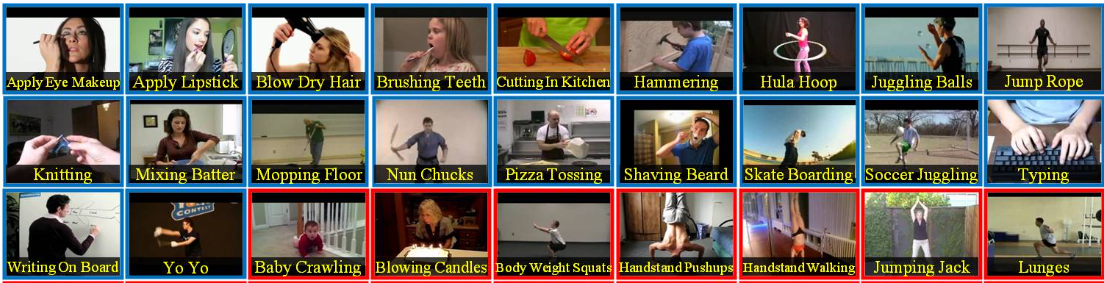
\includegraphics[scale=.5]{Images/Chapter4/ucf101.png}
	\caption[]{ نمونه‌ای از مجموعه‌داده‌ی \lr{UCF101}\cite{ucf101}   }
	\label{fig.41}
\end{figure}
دسته‌های موجود در \lr{UCF101} به پنج گروه کلی تقسیم می‌شوند:
\begin{enumerate}
	\item \textbf{‌فعالیت‌های ورزشی} 
	\item \textbf{فعالیت‌های تعاملی انسان با اشیا} 
	\item \textbf{فعالیت‌های تعاملی انسان با انسان} 
	\item \textbf{فعالیت‌های بدنی عمومی} 
	\item \textbf{فعالیت‌های نواختن موسیقی} 
\end{enumerate}

ویژگی مهم این مجموعه‌داده، تنوع بالای آن در شرایط تصویربرداری و پیچیدگی حرکات است 
که آن را به یک معیار معتبر برای ارزیابی مدل‌های تشخیص حرکات‌های انسانی و یادگیری پیوسته تبدیل می‌کند. نمونه‌هایی از داده‌های این مجموعه‌داده در \cref{fig.41} قابل مشاهده است. 
‌\subsection{مجموعه‌داده‌ی \lr{HMDB51}}
مجموعه‌داده \lr{HMDB51} \cite{hmdb51} یکی از مجموعه‌داده‌های پرکاربرد در زمینه‌ی تشخیص حرکات انسانی در ویدیو است که برای ارزیابی عملکرد الگوریتم‌های تشخیص حرکت طراحی شده است. 
این مجموعه شامل \lr{6{,}766} ویدیو در \lr{51} دسته‌ی فعالیت انسانی است که هر دسته تقریباً ۱۰۰ نمونه دارد. 
نمونه‌های موجود در \lr{HMDB51} از منابع متنوعی همچون فیلم‌های سینمایی، ویدیو‌های اینترنتی و فیلم‌های خانگی جمع‌آوری شده‌اند 
و طیف وسیعی از حرکات انسانی شامل فعالیت‌های بدنی، تعامل انسان با اشیاء و تعامل انسان با انسان را پوشش می‌دهند. یکی از ویژگی‌های مهم این مجموعه‌داده، تنوع بالا در صحنه، پس‌زمینه، زاویه دوربین و کیفیت ویدیوها است 
که تشخیص حرکات را به یک چالش واقعی تبدیل می‌کند. 
\begin{figure}
	\centering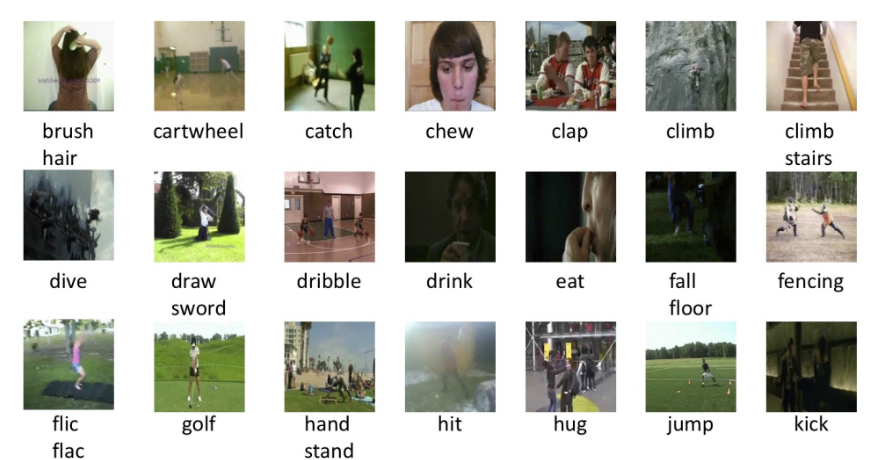
\includegraphics[scale=.6]{Images/Chapter4/HMDB_snapshot1-300x225.png}
	\caption[]{ نمونه‌ای از مجموعه‌داده‌ی \lr{HMDB51}\cite{hmdb51}   }
	\label{fig.42}
\end{figure}
به دلیل اندازه متوسط و تنوع مناسب، \lr{HMDB51} به‌طور گسترده برای آموزش و ارزیابی مدل‌های تشخیص حرکات و یادگیری پیوسته مورد استفاده قرار می‌گیرد. فعالیت‌های موجود در \lr{HMDB51} را می‌توان در پنج گروه کلی دسته‌بندی کرد:
\begin{enumerate}
	\item \textbf{فعالیت‌های عمومی صورت}
	\item \textbf{فعالیت‌های صورت همراه با تعامل با اشیا} 
	\item \textbf{حرکات عمومی بدن} 
	\item \textbf{حرکات بدن همراه با تعامل با اشیا} 
	\item \textbf{حرکات بدن در تعامل انسان با انسان} 
\end{enumerate}
نمونه‌ای از این داده‌ها در \cref{fig.42} قابل مشاهده است.
\section{تنظیمات آزمایش}
آزمایش‌ها بر روی دو مچموعه‌داده‌ی \lr{HMDB51}\cite{hmdb51} و \lr{UCF101}\cite{ucf101} به صورت جداگانه اجرا شده و در هر دو حالت، مدل پایه‌ی مورد استفاده، \lr{Open-VCLIP} \cite{open-vclip} می‌باشد که در فرآیند آموزش از وزن‌های پیش‌آموخته‌ی \lr{CLIP} \cite{clip} (نسخه‌ی \lr{ViT-B/16}) بهره برده است. آموزش با نرخ اولیه‌ی یادگیری $3.33 \times 10^{-6}$ (مقدار معین شده در تنظیمات \lr{Open-VCLIP}) تست گردید اما به علت یادگیری آهسته و دریافت نتیجه‌ی نامطلوب، نرخ اولیه‌ی یادگیری، بعد از آزمایش‌های مختلف، با مقدار $1.5 \times 10^{-3}$ برای مجموعه‌داده‌ی \lr{UCF101} و $1.5 \times 10^{-2}$ برای مجموعه‌داده‌ی \lr{HMDB51} مورد استفاده قرار گرفت. مجموعه‌داده‌ها به نسبت‌های $60\%$ برای آموزش، $30\%$ برای آزمون و $10\%$ برای اعتبارسنجی تقسیم شدند. تعداد وظیفه‌‌ برای هر اجرا، $10$ در نظر گرفته شد. تنظیمات مربوط به پرامپت، شامل طول هر پرامپت، مقدار بیشینه‌ تعداد پرامپت انتخابی در هر اجرا، به ترتیب 5 (طبق مقداردهی \lr{L2P} \cite{l2p})و 2 در نظر گرفته شده است.  طول استخر پرامپت متناسب با سناریوی استفاده شده، متفاوت خواهد بود. سایر تنظیمات، مانند تنظیمات معرفی شده در \lr{Open-VCLIP}، در نظر گرفته شده‌اند. در ادامه تنظیمات اجرا برای هر دو مجموعه‌داده‌ی مذکور بررسی خواهند شد. سخت افزار استفاده شده در این تحقیق، \lr{GPU L40S} با $48$ گیگابایت حافظه‌ی رم می‌باشد. 
\subsection{آزمایش با مجموعه‌داده‌ی \lr{UCF101}}
در این آزمایش ابتدا تعداد $5$ ایپاک برای هر وظیفه در نظر گرفته شد و پس از بررسی نمودار صحت بر حسب ایپاک طی شده، مشاهده شد که صحت وظایف پس از سه ایپاک چه در اعتبارسنجی و چه در آموزش ثابت می‌شوند. بنابراین ایپاک نهایی برای این مجموعه‌داده، $3$ در نظر گرفته شد. آزمایش این مجموعه‌داده در سه سناریو بررسی شد که در ادامه توضیح داده خواهد شد: 
\begin{enumerate}
	\item \textbf{استخر ثابت با جریمه‌ی وزن‌های پیشین:} 
	دراین حالت طول استخر پرامپت ثابت خواهد بود که در این آزمایش، به اندازه‌ی $202$ مقداردهی شده است. تعداد تکرار انتخاب هر پرامپت در یادگیری پیوسته، ذخیره می‌شود و هنگام انتخاب پرامپت در وظیفه‌ی جدید، متناسب با تعداد تکرار هر پرامپت، جریمه‌ای در نظر گرفته می‌شود. بنابراین احتمال انتخاب پرامپت‌های پیشین، تا حدودی کاهش می‌یابد(الگو گرفته از روش اضافه‌ی ذکر شده در \lr{L2P} \cite{l2p}).  
	\item \textbf{استخر پویا با مقداردهی تصادفی:}
	در این حالت طول استخر پرامپت اولیه به اندازه‌ی $20$ در نظر گرفته شده است. هر وظیفه‌‌ که اضافه می‌شود، به طول استخر $20$ واحد اضافه می‌شود. نکته‌ی حائز اهمیت در سناریوی فعلی و بعدی، این است که پرامپت‌های استفاده شده در وظایف قبلی، هنگام یادگیری وظیفه‌ی جدید، منجمد شده و صرفا قابلیت انتخاب شدن، دارند و تغییری نخواهند کرد. 
	\item \textbf{استخر پویا با مقداردهی مبتنی بر کدگذار متن \lr{CLIP}:}
	در این حالت، همه‌ی تنظیمات به جز مقداردهی اولیه‌ی کلید‌های استخر پرامپت، مانند سناریوی قبلی می‌باشد. به ازای هر دسته‌ در هر وظیفه، دو عدد کلید مقداردهی اولیه می‌شود به این صورت که برچسب هر دسته به همراه عبارت‌های معنی دار ثابت، از کدگذار متن مدل \lr{CLIP} عبور کرده و ویژگی‌های بدست آمده در کلیدها قرار می‌گیرند. به عنوان مثال اگر برچسب یک ویدیو، \lr{jumping person}  باشد، عبارتی که وارد کدگذار می‌شود برابر با \lr{\texttt{"a video of jumping person."}} خواهد بود. در این سناریو، مقادیر اولیه‌ی کلیدها معنادار بوده و نتایج نشان داده اند که تاثیر مثبتی در انتخاب درست پرامپت‌ها داشته‌اند.
\end{enumerate}

\subsection{آزمایش با مجموعه‌داده‌ی \lr{HMDB51}}
یش ابتدا تعداد $5$ ایپاک برای هر وظیفه در نظر گرفته شد و پس از بررسی نمودار صحت بر حسب ایپاک طی شده، مشاهده شد که یادگیری به خوبی صورت نگرفته است. بنابراین پس از افزایش ایپاک‌ها در طی آزمایش، ایپاک نهایی برای این مجموعه‌داده، $7$ در نظر گرفته شد. مانند مجموعه‌داده‌ی پیشین، آزمایش این مجموعه‌داده نیز در سه سناریو بررسی شد که در ادامه توضیح داده خواهد شد: 
\begin{enumerate}
	\item \textbf{استخر ثابت با جریمه‌ی وزن‌های پیشین:} 
	این سناریو نیز مانند توضیحات ذکر شده در قسمت قبل، اجرا شده است با این تفاوت که طول استخر پرامپت در این جا $102$ در نظر گرفته شده است.   
	\item \textbf{استخر پویا با مقداردهی تصادفی:}
	در این حالت طول استخر پرامپت اولیه ابتدا به اندازه‌ی $10$ در نظر گرفته شد و سپس به علت کسب نتیجه‌ی بهتر، به $25$ تغییر داده شد. هر وظیفه‌‌ که اضافه می‌شود، به طول استخر $25$ واحد اضافه می‌شود. نکته‌ی حائز اهمیت در سناریوی فعلی و بعدی، این است که پرامپت‌های استفاده شده در وظایف قبلی، هنگام یادگیری وظیفه‌ی جدید، منجمد شده و صرفا قابلیت انتخاب شدن، دارند و تغییری نخواهند کرد. 
	\item \textbf{استخر پویا با مقداردهی مبتنی بر کدگذار متن \lr{CLIP}:}
	همانند آن‌چه در بخش قبل گفته شد، تنظیمات مانند سناریوی پیشین باقی می‌مانند و صرفا مقداردهی اولیه‌ی کلیدها با کدگذار \lr{CLIP} صورت می‌گیرد. 
\end{enumerate}






























